% No modificar estas líneas de código, por favor dirigirse a INTRODUCCIÓN 
\newpage
\phantomsection\addcontentsline{toc}{section}{INTRODUCCIÓN} 

%------------------------
%
%       INTRODUCCIÓN
%
%------------------------

\section*{INTRODUCCIÓN}
En la industria moderna, el uso de autoclaves es esencial para garantizar procesos de esterilización y tratamiento térmico que cumplan con altos estándares de calidad y seguridad. La empresa \acrfull{itm}, ubicada en Cochabamba, provee, capacita y brinda servicio técnico de sus autoclaves a hospitales de distintos niveles en la ciudad, siendo su rendimiento fundamental para el correcto funcionamiento de la esterilización de materiales e instrumentos quirúrgicos. Sin embargo, la gestión eficiente de estos equipos representa un desafío constante, ya que requieren mantenimiento regular para evitar fallos inesperados que puedan afectar la producción.

Contar con un sistema de monitoreo remoto para las autoclaves podría transformar la eficiencia operativa de \acrshort{itm}. A través de la recolección y análisis en tiempo real de datos de funcionamiento, como temperatura, presión y ciclos de operación, sería posible anticipar fallas y realizar un mantenimiento preventivo más preciso. Esto no solo reduciría la necesidad de intervenciones correctivas costosas, sino que también optimizaría los tiempos de inactividad, garantizando que los procesos críticos se realicen sin interrupciones inesperadas.

Los beneficios de implementar un sistema de monitoreo remoto de autoclaves en \acrshort{itm} abarcan desde la reducción de costos operativos hasta la mejora en la productividad y en la capacidad competitiva de la empresa. Además, al permitir una supervisión constante, la empresa podría maximizar la vida útil de sus equipos y mejorar la calidad del producto final, adaptándose de manera más efectiva a las exigencias del mercado. Este proyecto tiene como objetivo explorar y diseñar una solución de monitoreo remoto que responda a estas necesidades, mejorando la operación y la sostenibilidad de \acrshort{itm} en un mercado cada vez más competitivo.

\subsection*{Antecedentes}
Las autoclaves son equipos de vital importancia en el ámbito de la salud, ya que garantizan la esterilización de instrumental y otros materiales mediante el uso de vapor a alta presión y temperatura. En Bolivia, muchos hospitales de segundo nivel dependen de la empresa \acrshort{itm} para el mantenimiento y re-acondicionamiento de estos dispositivos. Sin embargo, el modelo de mantenimiento tradicional que actualmente se aplica, conocido como mantenimiento correctivo, consiste en realizar intervenciones únicamente cuando los equipos presentan fallas evidentes, sin previsión de problemas futuros. Este enfoque tiene como consecuencia tiempos de inactividad prolongados, lo que impacta negativamente tanto en los costos operativos de \acrshort{itm} como en la disponibilidad de los autoclaves para los centros de salud.

En Europa, un proyecto similar de monitoreo remoto para autoclaves se implementó en hospitales de varios países para mejorar la gestión de los equipos de esterilización. Un ejemplo de ello es el sistema desarrollado en colaboración entre varias universidades e instituciones de salud, que permitió monitorizar parámetros críticos de las autoclaves como temperatura, presión y tiempos de ciclo en tiempo real. El uso de sensores \acrfull{iot} y la integración con plataformas de análisis predictivo permitió optimizar el mantenimiento, reduciendo los tiempos de inactividad y los costos asociados. Según \cite{Lopez2019}, este sistema no solo facilitó la monitorización remota, sino que mejoró la eficiencia operativa al permitir intervenciones preventivas antes de que se presentaran fallos críticos.

En Brasil, un proyecto de mantenimiento remoto de autoclaves fue implementado en una planta farmacéutica utilizando tecnologías \acrshort{iot} para mejorar la gestión de las autoclaves y predecir fallos. Este sistema permitía el monitoreo en tiempo real de las variables críticas, enviando los datos a una plataforma centralizada desde donde los técnicos podían detectar irregularidades antes de que se produjeran daños graves. Según \cite{Santos2020}, el sistema permitió la optimización de los recursos, ya que las intervenciones se hacían solo cuando era necesario, reduciendo significativamente los costos de mantenimiento correctivo y mejorando la disponibilidad operativa de los equipos.

\subsection*{Identificación del problema}
La empresa \acrshort{itm} se encarga de reacondicionar y dar mantenimiento a equipos que presentan fallas en 23 centros de salud de primer nivel ambulatorios, 7 integrales y 3 hospitales de segundo nivel en el municipio de cercado, ademas de estar a cargo de los equipos proporcionados en todo el país de Bolivia. Actualmente, el área de mantenimiento de \acrshort{itm} enfrenta desafíos para optimizar la gestión del mantenimiento de estos equipos, debido a que dependen principalmente de un modelo correctivo en el cual las intervenciones solo se realizan una vez que aparecen fallas evidentes. Esta situación provoca tiempos de inactividad no planificados donde estos dispositivos están fuera de servicio, lo cual incrementa los costos operativos y limita la capacidad de anticiparse a problemas que pueden afectar la seguridad y continuidad del servicio.

Para mejorar la confiabilidad y disponibilidad de las autoclaves, la empresa \acrshort{itm} ha propuesto implementar un modelo de mantenimiento predictivo. Sin embargo, enfrenta dificultades para llevarlo a cabo debido al acceso limitado a datos en tiempo real sobre el rendimiento y estado operativo de estos equipos, lo cual restringe su capacidad para anticipar fallas y optimizar la planificación de intervenciones.


En la siguiente Figura \ref{fig:arbol} se presenta el árbol de problema elaborado para la formulación del problema.

        \begin{figure}[!htb]
            \centering
            \caption{Árbol de problema} % Título de figura
            {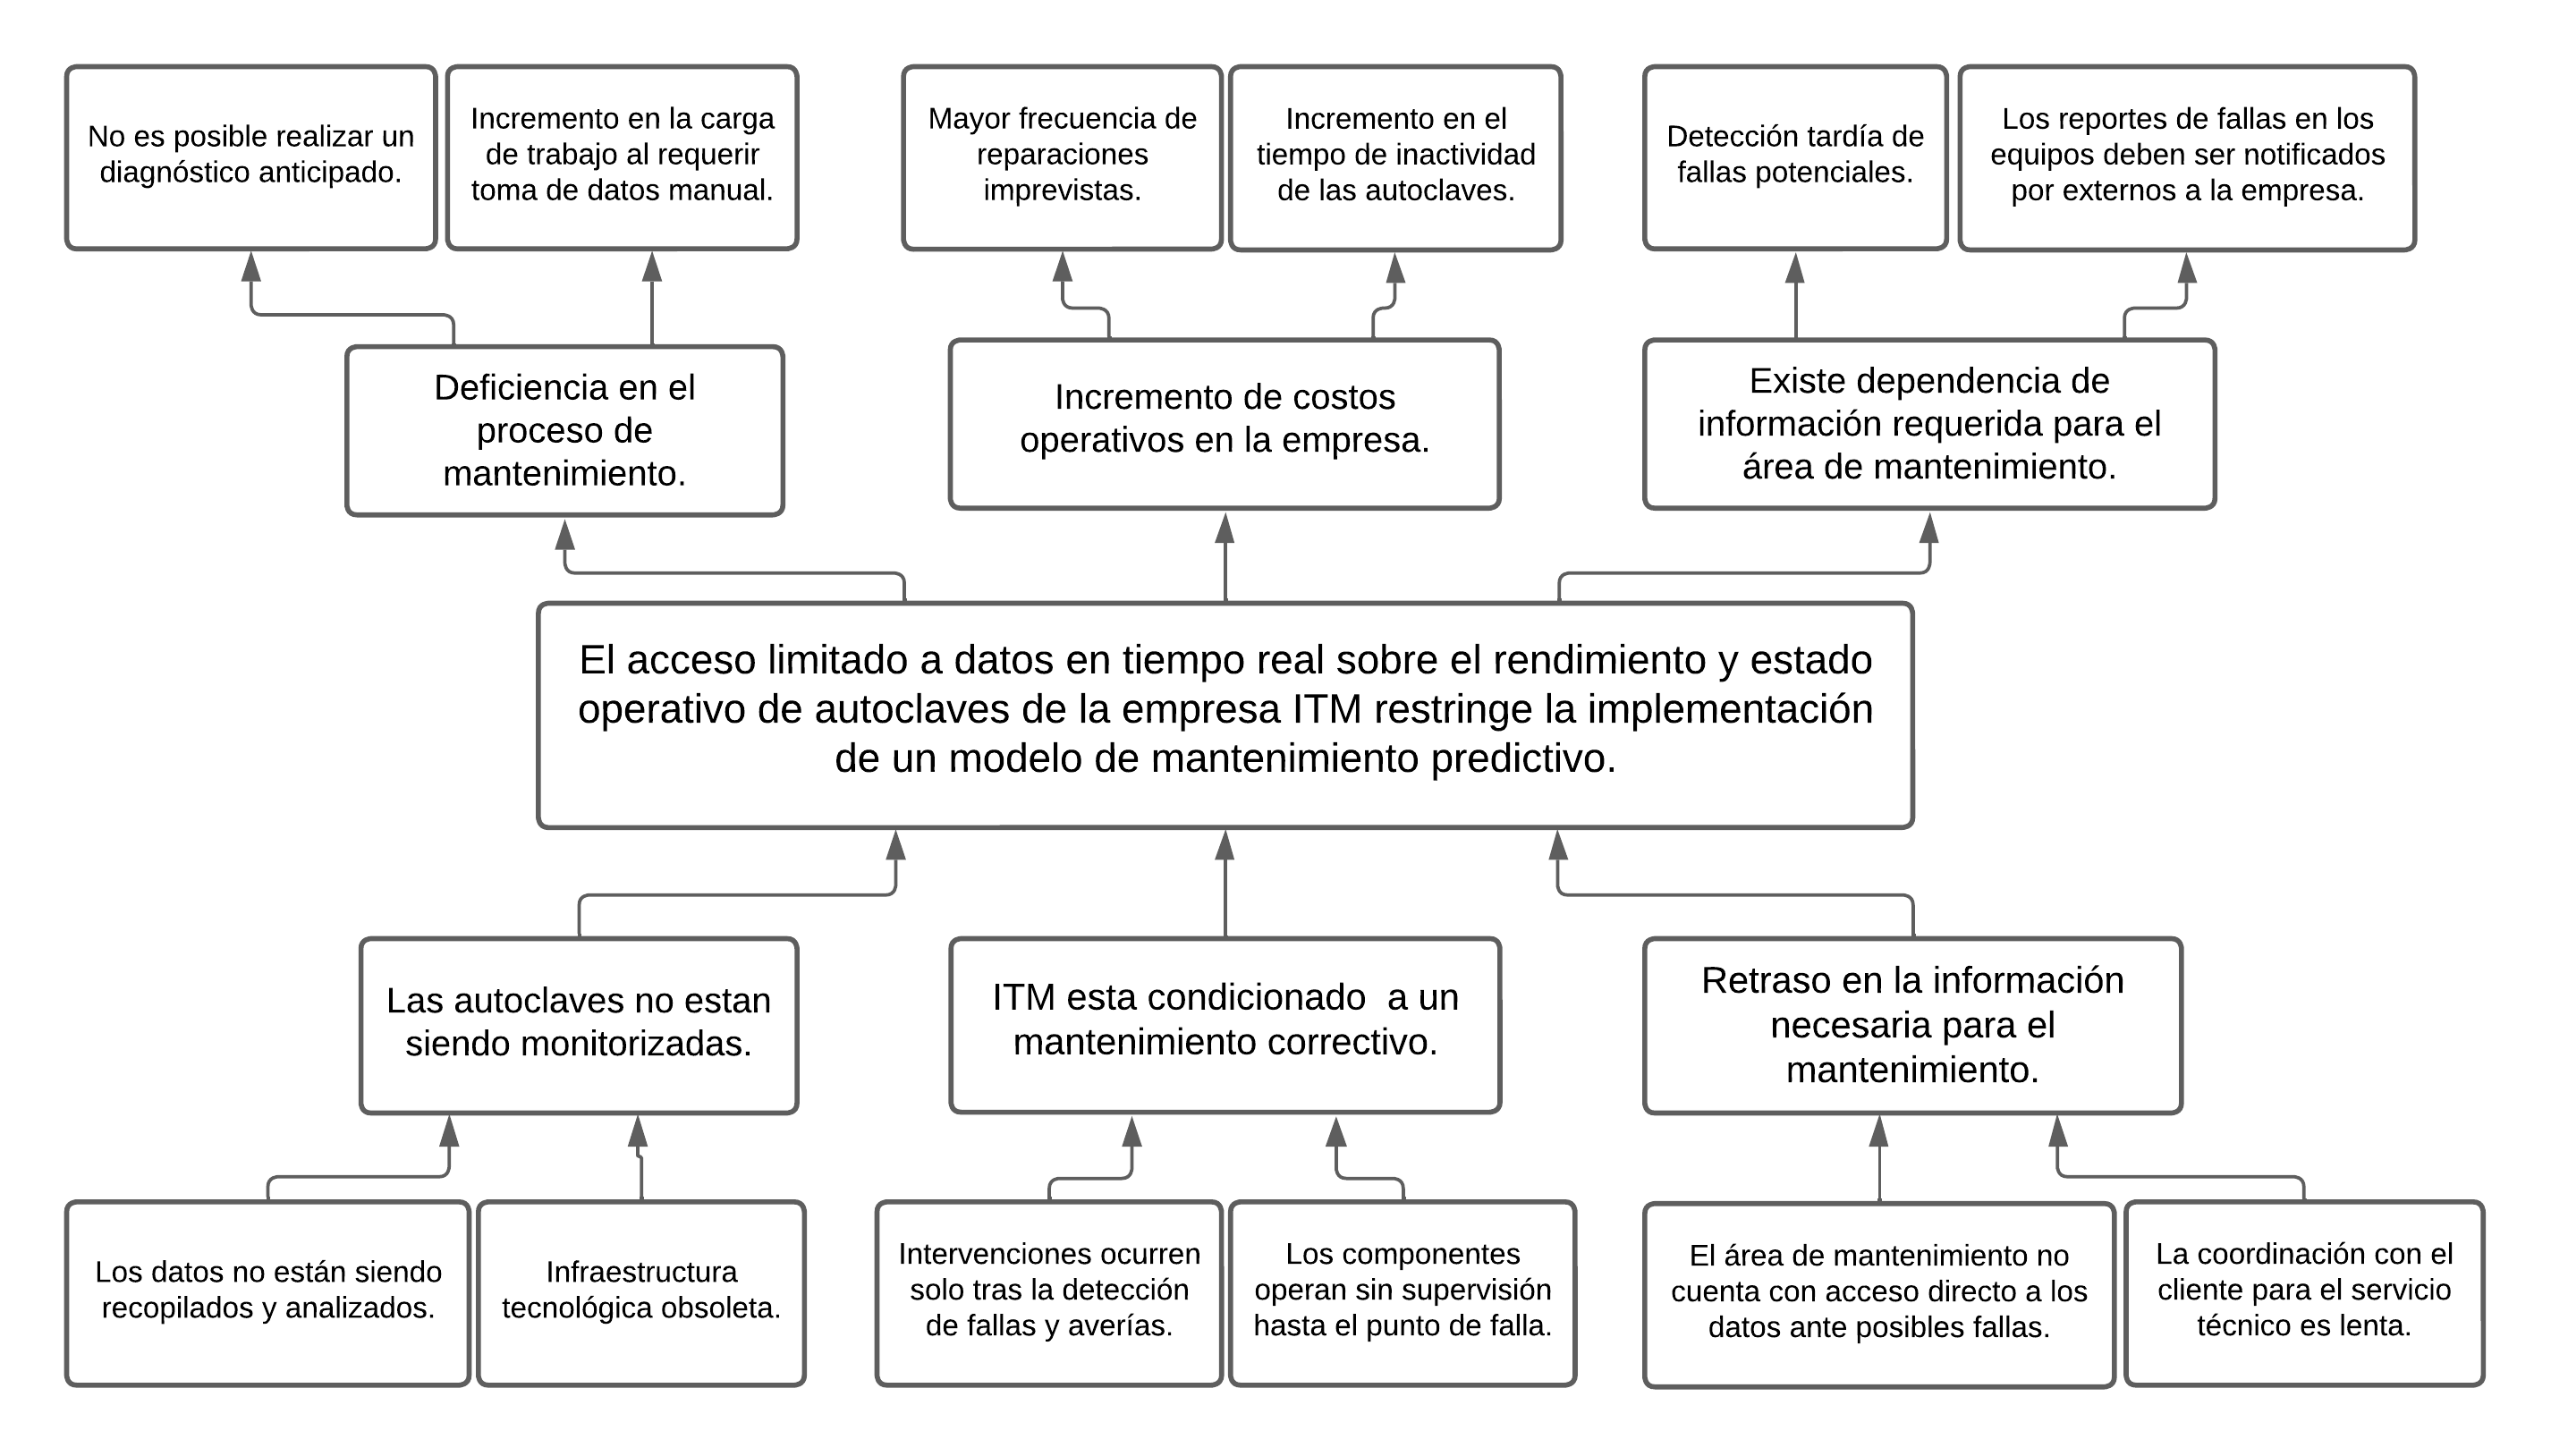
\includegraphics[width=1\columnwidth]{Figuras/arbol.png}}
             \centering{\textbf{Fuente:} Elaboración propia (2024)} % Fuente
            \label{fig:arbol}
        \end{figure}
 
\subsection*{Formulación del problema}
¿Qué solución tecnológica debería implementar la empresa \acrshort{itm} para garantizar el acceso en tiempo real al estado operativo de sus autoclaves e impulsar la transición hacia un modelo de mantenimiento predictivo?
 
\subsection*{Objetivos}
Para la elaboración del proyecto se plantea los siguientes objetivos:
\subsubsection*{Objetivo general}

Implementar un sistema de monitoreo y operación en tiempo real para autoclaves de la empresa \acrshort{itm} mediante tecnología \acrshort{iot}.

\subsubsection*{Objetivos específicos}

\begin{itemize}
\item Determinar los requerimientos técnicos y funcionales para la implementación del sistema de monitoreo de autoclaves.
\item Desarrollar la aplicación web que permita la visualización y gestión en tiempo real del estado de las autoclaves.
\item Establecer una infraestructura segura para la transmisión y almacenamiento de datos desde las autoclaves hasta la plataforma central de monitoreo.
\item Integrar el dispositivo \acrshort{iot} en las autoclaves para la recolección y transmisión continua de datos en tiempo real.
\item Validar los resultados de pruebas de funcionalidad del sistema en ambientes controlados.
\end{itemize}

\subsection*{Justificación}
A continuación se presentarán diversos puntos organizados en categorías que respaldan el desarrollo del proyecto.

\subsubsection*{Tecnológica}

La implementación de un sistema de mantenimiento predictivo para autoclaves se justifica debido a la necesidad de mejorar la eficiencia y efectividad en el mantenimiento en la empresa \acrshort{itm}. Según investigaciones recientes, el uso de tecnologías de \acrshort{iot} en la industria permite recopilar datos en tiempo real y detectar patrones de funcionamiento anómalos antes de que ocurran fallos críticos, lo cual reduce costos de mantenimiento y tiempo de inactividad \citep{J_tecnologica}. En particular, los sistemas de monitoreo remoto en equipos industriales han demostrado aumentar significativamente la precisión en el diagnóstico y la planificación de mantenimiento, lo que resulta en una operación más segura y rentable \citep{J_tecnologica2}. Por ello, la adopción de un sistema basado en \acrshort{iot} para el monitoreo de autoclaves en \acrshort{itm} permitirá una optimización en la gestión de datos sobre el estado de estos equipos, aumentando la eficiencia operativa y reduciendo los costos asociados a fallos inesperados.
\subsubsection*{Social}

La mejora en el acceso a datos en tiempo real representa un beneficio social significativo, debido a que facilita un mantenimiento predictivo más eficaz, asegurando la disponibilidad y seguridad de los equipos que son esenciales en industrias como la médica y la alimentaria, donde las autoclaves juegan un rol crítico. Según \cite{McKinsey2017}, el mantenimiento predictivo basado en datos en tiempo real puede reducir significativamente el riesgo de fallos, lo cual no solo prolonga la vida útil del equipo, sino que también protege a los trabajadores y asegura la continuidad en los procesos esenciales \citep{McKinsey2017}. Además, un acceso eficiente a la información permite tomar decisiones rápidas y fundamentadas, lo cual contribuye a una mayor seguridad y confianza tanto para los operadores como para las comunidades que dependen de estos servicios \citep{WEF2018}. Entonces podríamos decir que un sistema de acceso en tiempo real para autoclaves mejora las condiciones de trabajo y los resultados para el usuario final, en nuestro caso los hospitales con los que trabaja \acrshort{itm}.

\subsubsection*{Económica}
La implementación de un sistema de monitoreo de datos en tiempo real para mejorar el mantenimiento predictivo, presenta beneficios significativos que aporta en la reducción de costos operativos y de mantenimiento. Estudios muestran que el mantenimiento predictivo, en comparación con el mantenimiento reactivo o preventivo tradicional, puede reducir los costos de mantenimiento hasta en un 20-30\% al disminuir la frecuencia de reparaciones no planificadas y optimizar la utilización de recursos \citep{Mobley2002}. Además, al detectar y abordar posibles fallas de manera anticipada, se minimizan las interrupciones en la producción, lo cual reduce las pérdidas económicas asociadas con el tiempo de inactividad de los equipos \cite{Schneider2015}. Al permitir un mantenimiento predictivo más preciso, se reduce la necesidad de intervenciones correctivas, el proyecto no solo mejora la eficiencia operativa, sino que también se traduce en un ahorro económico significativo para la empresa a mediano y largo plazo.

\subsection*{Alcance}
\begin{itemize}
    \item El proyecto se centrará únicamente en autoclaves de sobremesa y no abordará otros tipos de equipos de esterilización.
    \item El proyecto no abarcará un análisis de datos obtenidos de las autoclaves para completar el modelo de mantenimiento predictivo, se enfocará unicamente en la recolección de datos garantizando su integridad en el envío.
    \item El proyecto se implementará únicamente en los centros de salud y hospitales que gestiona \acrshort{itm}.
    \item La evaluación del impacto del sistema se realizará durante un período de seis meses tras la implementación, lo que limitará la capacidad de evaluar efectos a largo plazo.
    \item El proyecto considerará la selección de proveedores externos para la implementación del sistema \acrshort{iot}, no limitándose así a los recursos internos de \acrshort{itm}.
    \item El estudio se centrará en los operadores de autoclaves y el personal de salud a cargo del sistema.
\end{itemize}

\subsection*{Límites}

\begin{itemize}
    \item El proyecto no se implementará en hospitales de tercer nivel.
    \item Se cuenta con solo un semestre académico para el desarrollo del proyecto.
    \item No se tiene la disponibilidad de autoclaves para realizar pruebas puesto que están en funcionamiento en hospitales, unicamente se tiene disponible aquellas que están para reacondicionamiento.
    \item El proyecto tiene un presupuesto limitado, lo que restringe la adquisición de tecnologías de \acrshort{iot} más avanzadas.
    \item La investigación no incluirá un análisis exhaustivo de las regulaciones y normativas sobre el reacondicionamiento de autoclaves, enfocándose en el desarrollo técnico del sistema \acrshort{iot}.
\end{itemize}
